\chapter{Grundlegende Funktionen}

\section{Signale}

\subsection{Sprungfunktion}

\[ 
	\sigma(t) := \left\{
		\begin{array}{c c}
			1 & t \geq 0 \\
			0 & t \leq 0
		\end{array}
		\right.
\]

\begin{figure}[h!]
	\centering
	\begin{tikzpicture}
		% zeichne Koordinatensystem
		\draw[->] (-2,0) -- (4,0) node[anchor=north] {$t$};
		\draw[->] (0,0) -- (0,2) node[anchor=east] {$u(t)$};
		
		% zeichne Labels
		\draw (0,0) node[anchor=north] {$0$};
		\draw (0,1) node[anchor=east] {$1$};
			
		% Zeigne Singalverlauf
		\draw[-, thick, red] (-1.5,0) -- (0,0) {};
		\draw[-, thick, red] (0,0) -- (0,1) {};
		\draw[-, thick, red] (0,1) -- (3.5,1) {};
	\end{tikzpicture}
	\caption{Sprungfunktion}
	\label{fig:sprungfunktion}
\end{figure}


\subsection{Rechteckimpuls}

\[ 
	u(t) = \left\{
		\begin{array}{c c}
			A & t_0 \leq t \leq t_1 \\
			0 & t_1 < t < t_0
		\end{array}
		\right.
\]

\begin{figure}[h!]
	\centering
	\begin{tikzpicture}
		% zeichne Koordinatensystem
		\draw[->] (-2,0) -- (4,0) node[anchor=north] {$t$};
		\draw[->] (0,0) -- (0,2) node[anchor=east] {$u(t)$};
		
		% zeichne Labels
		\draw (0,0) node[anchor=north] {$t_0$};
		\draw (2,0) node[anchor=north] {$t_1$};
		\draw (0,1) node[anchor=east] {$A$};
			
		% Zeigne Singalverlauf
		\draw[-, thick, red] (-1.5,0) -- (0,0) {};
		\draw[-, thick, red] (0,0) -- (0,1) {};
		\draw[-, thick, red] (0,1) -- (2,1) {};
		\draw[-, thick, red] (2,1) -- (2,0) {};
		\draw[-, thick, red] (2,0) -- (3.5,0) {};
	\end{tikzpicture}
	\caption{Rechteckimpuls}
	\label{fig:rechteckimpuls}
\end{figure}

\subsection{Rampenfunktion}

\[ 
	u(t) = \left\{
		\begin{array}{c c}
			t & t \geq 0 \\
			0 & t < 0
		\end{array}
		\right.
\]

\begin{figure}[h!]
	\centering
	\begin{tikzpicture}
		% zeichne Koordinatensystem
		\draw[->] (-2,0) -- (4,0) node[anchor=north] {$t$};
		\draw[->] (0,0) -- (0,2) node[anchor=east] {$u(t)$};
		
		% zeichne Labels
		\draw (0,0) node[anchor=north] {$0$};
			
		% Zeigne Singalverlauf
		\draw[-, thick, red] (-1.5,0) -- (0,0) {};
		\draw[-, thick, red] (0,0) -- (3.5,1.5) {};
	\end{tikzpicture}
	\caption{Rampenfunktion}
	\label{fig:rampenfunktion}
\end{figure}

\subsection{Dirac-Delta Funktion}

\[ 
	\widetilde{\sigma}(t, \Delta t) = \left\{
		\begin{array}{c c}
			1 & t > \Delta t \\
			\frac{1}{2} + \frac{t}{2 \cdot \Delta t} &
				- \Delta t \leq t \leq \Delta t \\
			0 & t < - \Delta t
		\end{array}
		\right.
\]

\begin{figure}[h!]
	\centering
	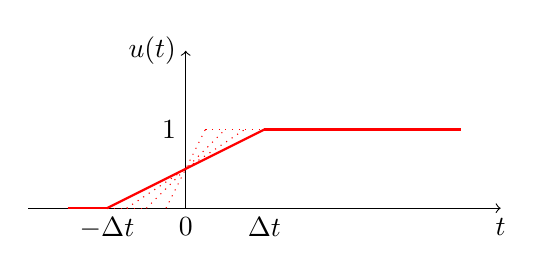
\begin{tikzpicture}
		% zeichne Koordinatensystem
		\draw[->] (-2,0) -- (4,0) node[anchor=north] {$t$};
		\draw[->] (0,0) -- (0,2) node[anchor=east] {$u(t)$};
		
		% zeichne Labels
		\draw (0,0) node[anchor=north] {$0$};
		\draw (0,1) node[anchor=east] {$1$};
		\draw (-1,0) node[anchor=north] {$- \Delta t$};
		\draw (1,0) node[anchor=north] {$\Delta t$};
			
		% Zeigne Singalverlauf
		\draw[-, thick, red] (-1.5,0) -- (-1,0) {};
		\draw[-, thick, red] (-1,0) -- (1,1) {};
		\draw[-, thick, red] (1,1) -- (3.5,1) {};

		%\draw[-, red, dotted] (-1.5, 0) -- (-0.75, 0) {};
		\draw[-, red, dotted] (-0.75, 0) -- (0.75, 1) {};
		%\draw[-, red, dotted] (0.75, 1) -- (3.5, 1) {};

		%\draw[-, red, dotted] (-1.5, 0) -- (-0.5, 0) {};
		\draw[-, red, dotted] (-0.5, 0) -- (0.5, 1) {};
		%\draw[-, red, dotted] (0.5, 1) -- (3.5, 1) {};

		\draw[-, red, dotted] (-1.5, 0) -- (-0.5, 0) {};
		\draw[-, red, dotted] (-0.25, 0) -- (0.25, 1) {};
		\draw[-, red, dotted] (0.25, 1) -- (3.5, 1) {};
	\end{tikzpicture}
	\caption{Dirac-Delta Funktion}
	\label{fig:dirac-delta}
\end{figure}

\[	
	\frac{d \widetilde{\sigma}(t)}{dt} = \left\{
		\begin{array}{c c}
			0 & t > \Delta t \\
			\frac{1}{2 \cdot \Delta t} &
				- \Delta t \leq t \leq \Delta t \\
			0 & t < - \Delta t
		\end{array}
		\right.
\]

\begin{figure}[h!]
	\centering
	\begin{tikzpicture}
		\usepgflibrary{patterns}
		% zeichne Koordinatensystem
		\draw[->] (-2,0) -- (4,0) node[anchor=north] {$t$};
		\draw[->] (0,0) -- (0,2) node[anchor=east] {$u(t)$};
		
		% zeichne Labels
		\draw (0,0) node[anchor=north] {$0$};
		\draw (-1,1) node[anchor=east] {$\frac{1}{2 \cdot \Delta t}$};
		\draw (-1,0) node[anchor=north] {$- \Delta t$};
		\draw (1,0) node[anchor=north] {$\Delta t$};
			
		% Zeigne Singalverlauf
		\draw[-, thick, red] (-1.5,0) -- (-1,0) {};
		\draw[-, thick, red] (-1,0) -- (-1,1) {};
		\draw[-, thick, red] (-1,1) -- (1,1) {};
		\draw[-, thick, red] (1,1) -- (1,0) {};
		\draw[-, thick, red] (1,0) -- (3.5,0) {};

		% Fläche einfärben
		\draw[pattern=north east lines, pattern color=gray] 
			(-1,0) rectangle (1,1);

		% Hinweis
		\draw[-] (0.5, 0.5) -- (2, 1) {};
		\draw (2,1) node[anchor=west] {$A=1$};
	\end{tikzpicture}
	\caption{Dirac-Delta Funktion}
	\label{fig:dirac-delta}
\end{figure}



\section{Eigneschaften}

\subsection{Gerade Funktionen}

\subsection{Ungerade Funktionen}

\subsection{Überlagerung}

\subsection{Stetigkeit}

\subsection{Sprungstetigkeit}
